% first example chapter
% @author Jan Robert Rösler 
%
\chapter{Entwurf}
In diesem Kapitel wird der vollständige Entwurf einer Steuerung für ein RC Fahrzeug dargestellt.
Für dieses Kapitel war besonders Buch des Erfinders von Keras, Francois Chollet, hilfreich \cite{chollet2018deep}.\\

Wie im vorangegangenen Kapitel erläutert, entstand die Idee für die Steuerung eines RC-Fahrzeuges mit Neuronalen Netzen im Kontext einer Arbeit der ETH Zürich.
<<<<<<< HEAD
Das dort entworfene DroNet wurde bereits kurz vorgestellt und wird die Basis für die neuronale Steuerung sein. 

DroNet ist ein 8-Layer Convolutional Neural Network, das hauptsächlich aus drei Residual-Blöcken besteht. Als Input bekommt das Netz ein 8-Bit Graustufenbild mit 200 x 200 Pixel. Es gibt zwei Outputs, einmal einen Lenkwinkel aus dem Intervall $\interval{-1}{1}$ und einmal die Kollisionswahrscheinlichkeit in Prozent. hierbei gilt, Werte~< 0 entsprechen einer Rechtskurve, Werte~> 0 einer Linkskurve.

DroNet hat \num{3.2e5} Parameter und schafft eine Verarbeitungsrate von 20 fps.
Wie im vorigen Kapitel bereits erwähnt, wurde DroNet auf einem frei verfügbaren Datensatz trainiert.\\
Im der Arbeit werden die Ergebnisse mit anderen Netzwerken verglichen, die mit dem selben Datensatz trainiert wurden. Anhand verschiedener Metriken zur Messung der Bestimmungsgenauigkeit, wird die Performance auf dem Datensatz bestimmt. Ein solcher Vergleich ist für diese Arbeit jedoch nicht durchgeführt, da ein konkretes Szenario untersucht wird.
\newpage 

\section{Hardware und Strecke}
\paragraph{Fahrzeug}
Das vom HAW-Team aufgebaute Fahrzeug für den Carolo-Cup \ref{img:Carolo-Fahrzeug}, besteht, abgesehen von Chassis, Motorelektronik und Servos, im Kern aus einem Intel \gls{ac:nuc}, auf dem die vollständige Bildverarbeitung und Logik berechnet wird und der Kamera, die die Bilder liefert. Der Prozessor ist ein Intel i5 der dritten Generation. Die Kamera ist eine \textsc{ueye} Schwarzweißkamera der Firma \gls{ac:ids}, die über USB mit dem NUC verbunden ist. 
Die Kontrolle per Fernsteuerung, zum Eingreifen im Fehlerfall und zum Positionieren des Fahrzeugs kommuniziert über Funk direkt mit dem Motorcontroller.\\
Auf dem Intel NUC ist ein Unix Betriebssystem eingerichtet.
Eine funktionsfähige Hardware Abstraktion für den Motor und die Steuerungsservos ist vom Carolo-Cup Team bereits entwickelt und steht mir im Weiteren zur Verfügung, diese ist in C++ implementiert.

\begin{figure}[h]
	\centering
	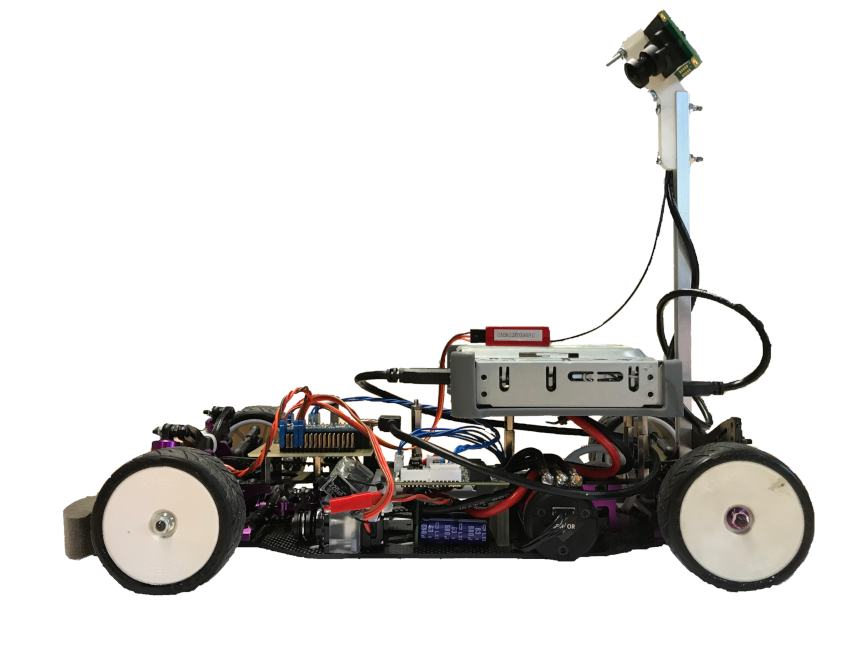
\includegraphics[scale=0.3]{figures/Fahrzeug.png}
	\caption{Das Carolo-Cup Fahrzeug}
	\label{img:Carolo-Fahrzeug}
\end{figure}

\paragraph{Strecke}
Die HAW Teststrecke ist ein Rundkurs mit verschiedenen Kurven und einem Kreuzungszenario. Die Länge der äußeren Fahrbahn beträgt 36,1 Meter, die innere Fahrbahn ist 31,3 Meter lang.\\
Die Fahrbahn mit weißen Band auf schwarzem Untergrund abgeklebt und entspricht der Erscheinung einer Straße, mit unterbrochener Mittellinie. Einige Besonderheiten der Strecke, wie zum Beispiel Parklücken, sind Teil der Aufgaben des Carolo-Cups, spielen in dieser Arbeit aber keine Rolle.
Die Abbildung~\ref{img:teststrecke} zeigt einen Ausschnitt der Fahrbahn, zu sehen ist eine fast kreisförmige Kurve und die Kreuzungssituation. 
Der Teststreckenraum ist fensterlos, es wurde sowohl bei Aufnahme der Trainingsbilder, als auch bei den Testfahrten darauf geachtet, dass die volle Deckenbeleuchtung an ist, um für optimale und gleichbleibende Beleuchtungsverhältnisse zu sorgen.

\begin{figure}[h]
	\centering
	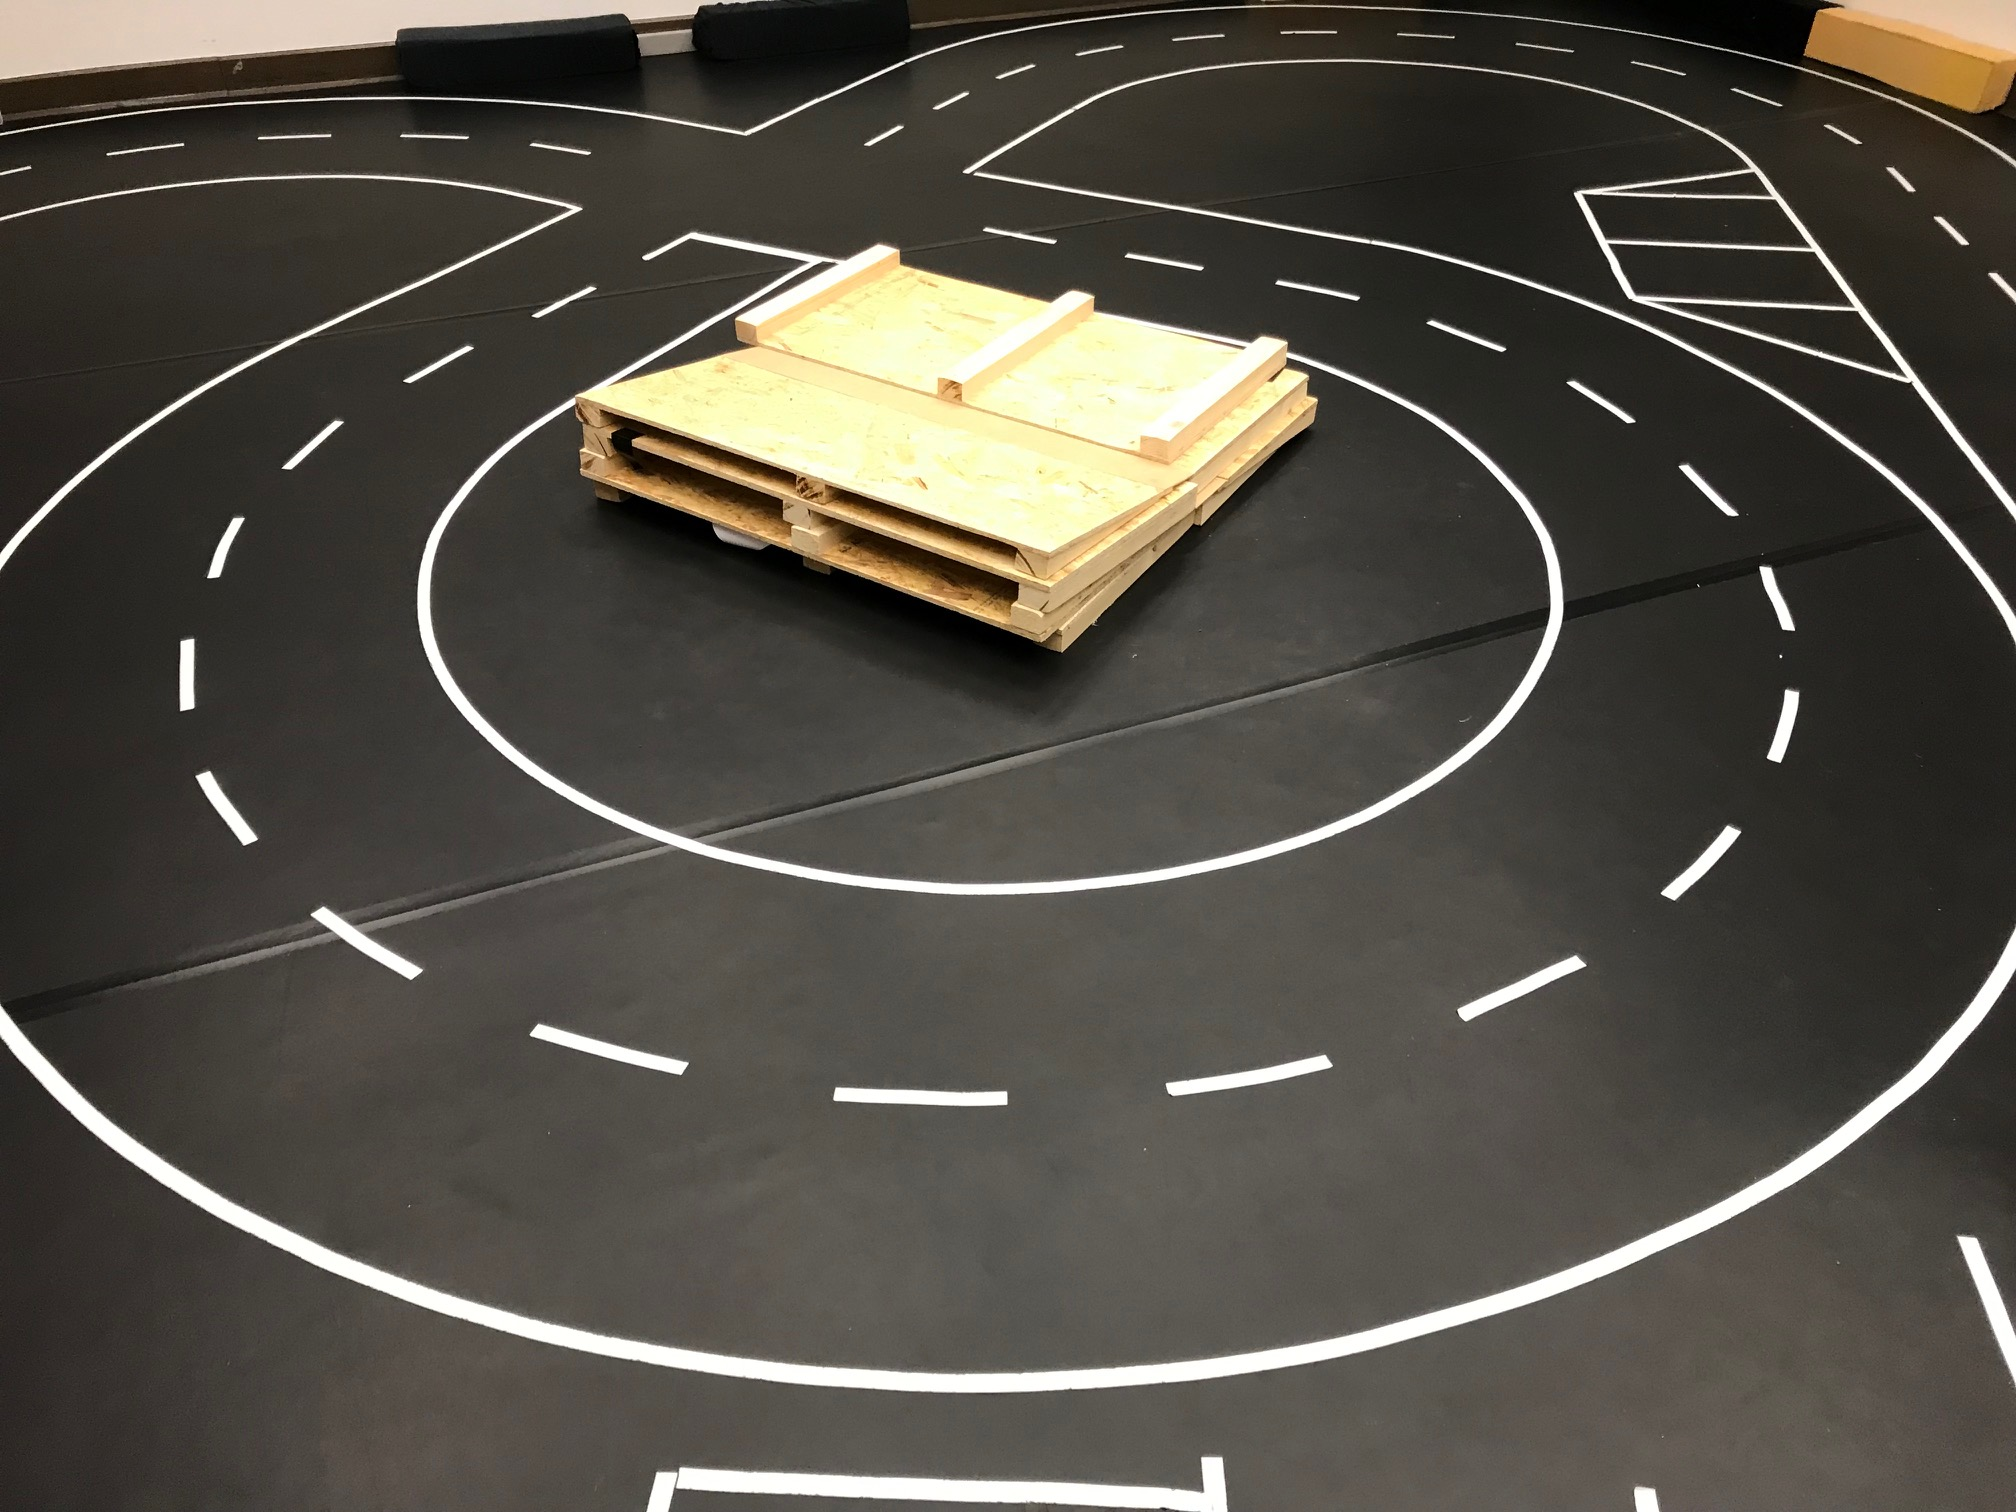
\includegraphics[scale=0.15]{figures/Teststrecke-Ausschnitt.jpg}
	\caption{Ein Ausschnitt der Teststrecke}
	\label{img:teststrecke}
\end{figure}
\paragraph{Rechnerhardware}
Bildverarbeitung und Training des Netzes werden auf einem Windows Computer (Windows 10) mit einer GeForce GTX 950 Grafikkarte berechnet. Da mit einer relativ kleinen Bildanzahl gearbeitet wird und das Neuronale Netz sehr kompakt in Hinblick auf die Parameteranzahl ist, wird keine High-end Grafikkarte benötigt.


\section{Trainingsdaten}

Um Trainingsdaten, also Bilder der Teststrecke mit dazugehörigem Lenkwinkel zu bekommen, wird auf einen Algorithmus eines Carolo-Cup Teams (\textsc{TeamWorstCase}) der HAW zurückgegriffen. Trainingsdaten per Hand zu generieren erwies sich als sehr schwierig, per Fernsteuerung lässt sich kaum sauber und kontinuierlich durch den Rundkurs steuern.

Auf mehreren Fahrten über den Rundkurs mit dem Algorithmus von \textsc{TeamWorstCase}, wurden über 20.000 Bilder gesammelt. Da die Steuerung nicht völlig sauber funktionierte und die Bildfolgen mehrfach Ausreisser enthielten, mussten Bilder per Hand aussortiert werden. Am Ende dieser Vorauswahl standen etwas über 6.000 Bilder für das Training zur Verfügung. Die Auflösung der Aufnahmen ist 752x480 Pixel. Die untere Hälfte der Bilder ist durch eine kamerainterne Vorverarbeitung bereits geschwärzt, \textsc{TeamWorstCase} hat für ihre weitere Verarbeitung so direkt den Teil des Bildes ausgeblendet, auf dem das Fahrzeug selbst zu sehen ist. Da dieser Teil des Bildes im weiteren ohnehin weggeschnitten wird, hat das keine Auswirkungen. 

Ein Beispiel aus diesen Fahrbahnaufnahmen zeigt Abbildung~\ref{img:rohbild}, die Aufnahme ist automatisch in Graustufen, da die Kamera nur in diesem Farbmodus aufnimmt.
Diese Rohdaten sind die Basis für das Training und müssen dazu einer Vorverarbeitung unterzogen werden. 

\begin{figure}[h]
	\centering
	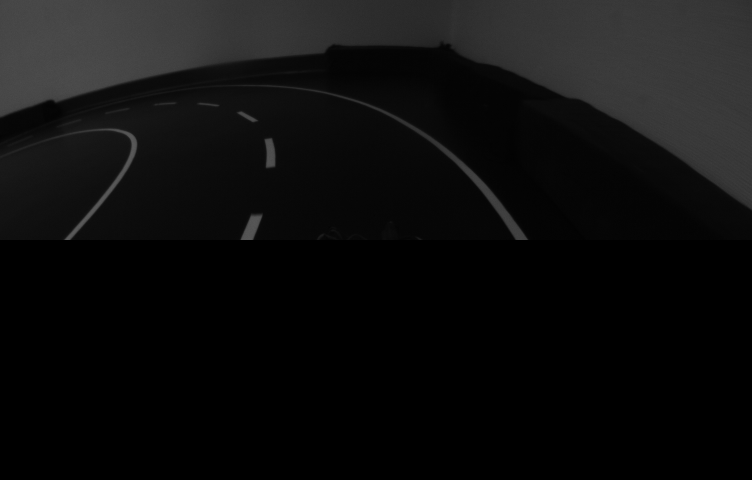
\includegraphics[scale=0.4]{figures/Rohbild.png}
	\caption{Kameraaufnahme der Fahrbahn}
	\label{img:rohbild}
\end{figure}


\section{Vorverarbeitung und Fine Tuning}

\subsection{Software}
Die Bildverarbeitung und das Training sind mit Python programmiert. Für Operationen auf Bildern wird die \gls{gl:opencv} Bibliothek verwendet. Das Neuronale Netz und die Struktur für Verarbeitung der Bilder und Training sind mit Keras implementiert.\\
Einzelne Funktionen zur Auswertung und für das Training sind aus dem Repository der DroNet Gruppe der ETH Zürich übernommen, diese sind im Code entsprechend kenntlich gemacht.

Die Abstraktion für den Motorcontroller auf dem Fahrzeug ist in C++ implementiert, die Steuerungskontrolle auf Fahrzeugseite ist daher in C entwickelt.\\
Die Python Module laufen auf einem Windows Computer in einer virtuellen Umgebung, die mit \gls{gl:anaconda} verwaltet wird. Es sind 2 Umgebungen mit Python 3.6.5 eingerichtet. Auf dem Fahrzeug (NUC) kommt zusätzlich \gls{ac:vscode} zum Einsatz, so wie eine Debugging Umgebung mit \gls{gl:pycharm} für die Python Module\\
Keras wird in Version 2.1.6 auf einem Tensorflow-Backend in Version 1.10.0 verwendet.

\subsection{Preprocessing}

Um die Bilder für das Training aufzubereiten, wird eine Verarbeitungspipeline eingerichtet, die in der gleichen Form auch für die Vorverarbeitung im Steuerungsmodus genutzt wird. Die Bilder, die das Netz zum Training zu \glqq sehen \grqq{} bekommt, sollen die gleiche Verarbeitung durchlaufen wie die Live-Bilder, die später zum Steuern benutzt werden.

\paragraph{Lenkwinkelskalierung}
Zunächst wird die Verteilung der Lenkwinkel betrachtet. Allerdings muss hier noch eine Skalierung erfolgen, denn die im Carolo-Cup-Fahrzeug verwendete Kodierung entspricht nicht der Kodierung, in der das neuronale Netz trainiert wurde. 

\begin{figure}[h]
	\centering
	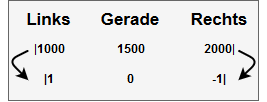
\includegraphics[scale=0.6]{figures/Lenkwinkelskalierung.png}
	\caption{Skalierung der Lenkwinkel-Wertebereiche}
	\label{img:skalierunglenkwinkel}
\end{figure}

Wie Abbildung~\ref{img:skalierunglenkwinkel} zeigt, müssen die Wertebereiche umgerechnet werden. Für jeden Lenkwinkel wird zunächst mit $(Wert-1500)/500$ auf den Bereich $\interval{0}{1}$ skaliert.t. Damit erhält man Werte im Intervall $\interval{-1}{1}$. Dabei wurde die Codierung der negativen Werte als Rechtslenkung und der positiven Werte als Linkslenkung beachtet..

\paragraph{Bilderset}
In Abbildung~\ref{fig:steuerungswinkel} ist die Lenkwinkelverteilung grafisch aufbereitet. Die x-Achse bildet den Lenkwinkel aus $\interval{-1}{1}$ ab, die y-Achse die Anzahl der Trainingsbilder mit dem jeweiligen Lenkwinkel. Grafik~\ref{fig:anglesa} zeigt die Verteilung der Lenkwinkel im Verhältnis zu der Anzahl der Bilder. Es wird sofort ersichtlich, dass die Mehrheit der gesammelten Lenkdaten von einer Fahrt geradeaus, mit Lenkwinkel um 0.0, stammen. Um eine möglichst ausgeglichene Verteilung zu erreichen wird eine Anpassung vorgenommen.

Alle Bilder, mit Ausnahme derer, die mit einem Lenkwinkel von 0.0 assoziiert sind, werden gespiegelt. So kann die Trainingsdatenmenge verdoppelt werden und gleichzeitig eine ausgeglichene Verteilung der Lenkwinkel erreicht werden. Grafik~\ref{fig:anglesb} zeigt die Verteilung nach der Anpassung.

Die Spiegelung sorgt automatisch dafür, dass Aufnahmen der rechten Fahrbahnseite zu Aufnahmen der Linken werden. Diese Erweiterung der Trainingsdaten auf beide Spuren wird aber nicht als Problem betrachtet, die Annahme ist, dass Fahrbahneigenschaften unabhängig der Fahrbahnseite gelernt werden können und das Training dadurch robuster wird. So entsteht ein Traningsbilder-Set von gut 11.000 Bildern.

\begin{figure}[h]
	\centering
	\begin{subfigure}{.5\textwidth}
	\centering
		  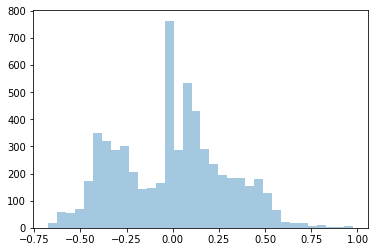
\includegraphics[width=1\linewidth]{figures/steeringAngleDistribution.png}
	 	  \caption{}
		  \label{fig:anglesa}
	\end{subfigure}%
	\begin{subfigure}{.5\textwidth}
	\centering
		  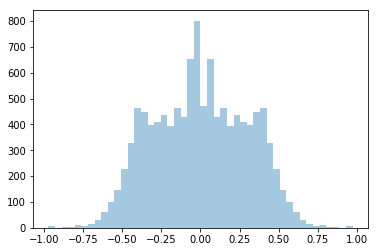
\includegraphics[width=1\linewidth]{figures/steeringAngleDistributionFlipped.png}
	 	  \caption{}
		  \label{fig:anglesb}
	\end{subfigure}%
	\caption{Lenkwinkelverteilung im Bilderset}
	\label{fig:steuerungswinkel}
\end{figure}%

Zu jedem Bild muss der dazugehörige Lenkwinkel als Label dem Lernprozess zur Verfügung gestellt werden. Beim Sammeln der Daten sind alle Parameter; Geschwindigkeit, Lenkwinkel und Framenummer in der Bildbezeichnung hinterlegt worden. Mit einer Parsing-Funktion wird die Bezeichnung gefiltert, die Lenkwinkel werden zusammen mit der Framenummer als eindeutigem Identifikator in einer Textdatei gespeichert. Die Textdatei wird für jeden Bildordner, Traning-, Validierung- und Testordner angelegt. Die Lenkdaten stehen somit direkt, auch für eine Analyse wie der oben erstellten Verteilung, zur Verfügung.

\paragraph{Bildverarbeitung}
Mit den so vorbereiteten Daten wird im Weiteren eine Pipeline mit Bildoperationen eingerichtet. Die Abbildung~\ref{fig:dronetfrozen} macht die Struktur der Verarbeitung deutlich.\\
Als Bildquellen kommen entweder die ueye-Kamera auf dem Fahrzeug in Frage, oder die Traningsdaten. Im einem ersten Schritt werden die Bilder skaliert und dann auf die Bildgröße 200x200 Bildpunkte zugeschnitten. Hier wurde speziell darauf geachtet, den Bildausschnitt mit dem größten Informationsgehalt zu erhalten, also möglichst viel der Fahrbahn im zugeschnittenen Bild.

Die Aufnahmen sind recht dunkel, selbst bei voll eingeschaltetem Raumlicht waren keine besseren Aufnahmen zu bekommen. Hier wird ein Histogrammausgleich für jedes Bild angewandt. Die Verteilung der Grauwerte wird so besser auf den gesamten Wertebereich aufgezogen, die Bilder werden heller.

Anschließend werden die Grauwerte auf den Wertebereich $\interval{0}{1}$ normalisiert. Für die Berechnung in CNNs ein üblicher Schritt, die Produkte der Multiplikationen bleiben in einem kleinen Wertebereich und ermöglichen so ein effizienteres Traning. Außerdem wird noch eine Umformung des Bildarrays von einem zweidimensionalen zu einem dreidimensionalen vorgenommen, dies ist im weiteren ebenfalls für die Verarbeitung im Netz von Bedeutung, auch wenn hier nur eine 1 für die eine Farbwertdimension (Grauwert) angefügt wird.

\begin{figure}[h]
	\centering
	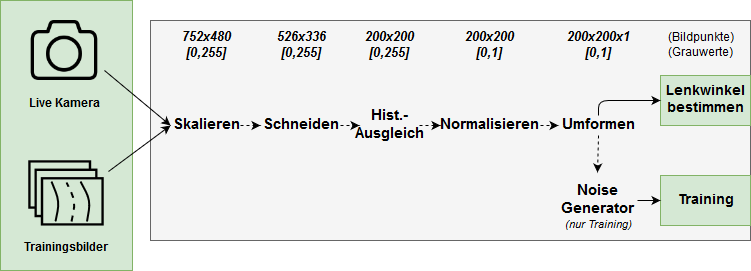
\includegraphics[scale=0.56]{figures/Pipeline.png}
	\caption{Bildverarbeitungsschritte}
	\label{fig:dronetfrozen}
\end{figure}

Für das Training wird auf einem Teil der Bilder ein Filter angewendet, der das Bild optisch rauschen lässt, um das Lernen robuster zu machen. Hierzu werden zufällige Werte aus einer (Gausschen-)Normalverteilung mit Mittelpunkt 0 gezogen und auf die Pixelwerte addiert. Für positive Werte werden die Pixel somit heller, für negative dunkler. So wird ein körniges, unscharfes Erscheinen des Bildes erreicht.\\
Darstellung~\ref{fig:pipelineexample} zeigt Auszüge aus den Bearbeitungsschritten, nach dem Zuschneiden, nach dem Histogrammausgleich und nach Durchlaufen eines Rausch-Filters.

\begin{figure}[h]
	\centering
	\begin{subfigure}{.33\textwidth}
	\centering
		  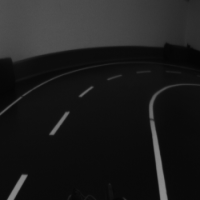
\includegraphics[width=0.9\linewidth]{figures/200x200.png}
	 	  \caption{}
		  \label{fig:imagea}
	\end{subfigure}%
	\begin{subfigure}{.33\textwidth}
	\centering
		  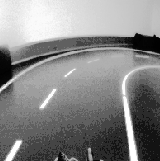
\includegraphics[width=0.9\linewidth]{figures/200x200Hist.png}
	 	  \caption{}
		  \label{fig:imageb}
	\end{subfigure}%
	\begin{subfigure}{.33\textwidth}
	\centering
		  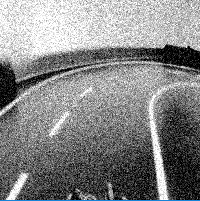
\includegraphics[width=0.9\linewidth]{figures/200x200Gauss.png}
	 	  \caption{}
		  \label{fig:imagec}
	\end{subfigure}%
	\caption{Beispiele verschiedener Bearbeitungsstufen, zugeschnitten (a), nach Histogrammausgleich (b) und nach Rausch-Filter (c) }
	\label{fig:pipelineexample}
\end{figure}%

Das Bilderset enthält jetzt gut 11.000 Bilder und muss für die Verwendung im Traningsprozess in Tranings- und Validierungsbilder aufgeteilt werden. Die hier verwendete Aufteilung ist im Verhältnis 1 zu 4. Damit entsteht ein Traningsbilderset mit 8.800 Bildern und ein Validierungsbilderset mit 2.200 Bildern.


\subsection{Fine Tuning}

\paragraph{Netzarchitektur}
Das CNN DroNet, welches als Grundlage verwendet wird, ist bereits mit Bildern von Fahrbahnen aus dem regulären Straßenverkehr trainiert. Eigenschaften einer Fahrbahn sind also, so die Annahme, bereits in der Gewichtsverteilung der einzelnen Layer repräsentiert. Die für diese Arbeit interessante Strecke fällt natürlich auch in die Kategorie Fahrbahn, allerdings unterscheiden sich die Aufnahmen der Teststrecke von denen, einer echten Fahrbahn. Es ist keine Bebauung vorhanden, ebenso gibt es keine anderen Verkehrsteilnehmer und die Art der Straßenführung unterscheidet sich von realen Situationen.

Statt die Gewichtsmatrizen des gesamten Netzwerkes anzupassen, wird nur ein Fine-Tuning des letzten Residual Blocks vorgenommen. Die architektonische Aufteilung in diese Blöcke ermöglicht ein gutes Aufteilen des Netzes in einen Teil mit festgesetzten bzw. eingefrorenen Gewichten und den Teil, der trainiert wird.

Abbildung~\ref{img:dronetfrozen} veranschaulicht diese Aufteilung. Der Teil des Netzes in roten Klammern wird vom Training ausgeschlossen, der grün eingeklammerte Block wird trainiert. Die Annahme ist, dass die ersten beiden Blöcke bereits allgemeine Eigenschaften einer Fahrbahn erlernt haben, die gut auf neue Szenarien generalisieren. Der letzte Residual Block enthält knapp $70\%$ der Parameter des gesamten Netzes. Die Annahme ist, das hier die allgemeinen Eigenschaften zu einer komplexeren Repräsentation zusammenwachsen, die gut auf die Testfahrbahn generalisiert. Darüberhinaus soll vermieden werden, dass das recht kleine Bilderset mit insgesamt 11.000 Bildern zu einer Überanpassung (Overfitting) führt. Das könnte auftreten, da die Aufnahmen auf Fahrsituationen der Teststrecke begrenzt sind, die keine große Heterogenität aufweisen. Nur einen Teil der Gewichte des Ntzes zu verändern, erscheint auch in diesem Kontext sinnvoll.

Zusätzlich wird die Ausgabe des Netzes verändert. Die Kollisionswahrscheinlichkeit spielt für diese Arbeit keine Rolle und die Traningsdaten enthalten keine entsprechenden Label, daher wird das entsprechende Ausgabe-Layer entfernt. Das Feedback für die Berechnung der Gewichtsanpassungen kommt nur vom Lenkwinkel.

\begin{figure}[h]
	\centering
	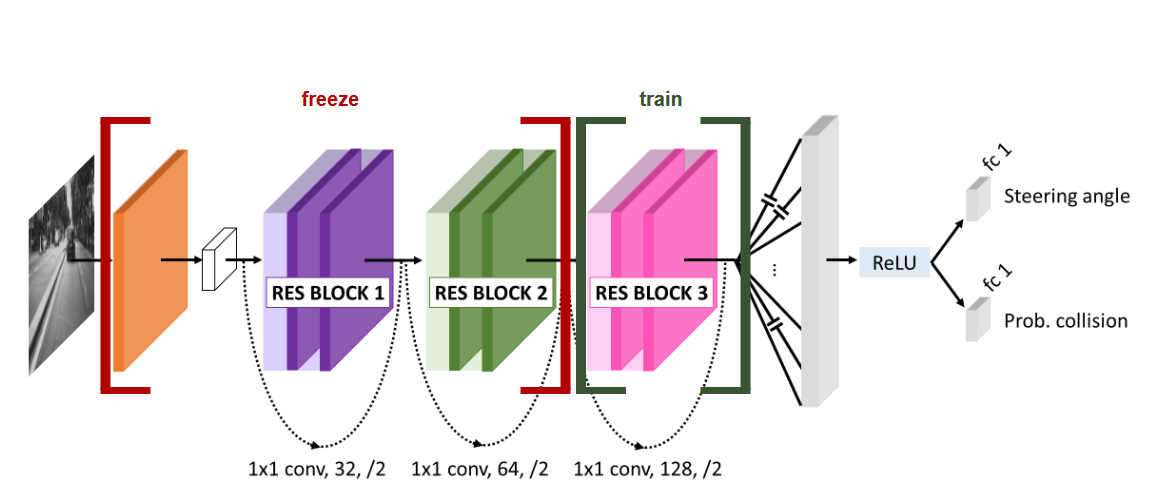
\includegraphics[scale=0.5]{figures/Architecture-DRONET-FROZEN.png}
	\caption{Angepasste Architektur}
	\label{img:dronetfrozen}
\end{figure}

\paragraph{Lernarchitektur}
Im Folgenden wird die Konfiguration für das Fine-Tuning vorgenommen und die Komponentenstruktur des Lernverfahrens erläutert.\\
Vor dem Fine-Tuning muss der Trainingsprozess konfiguriert werden, dafür werden vor dem Beginn die Hyperparameter festgelegt.

Das \gls{gl:adam} Optimierungsverfahren \cite{kingma2014adam} wird als Optimierungsalgortihmus aus dem DroNet Traning übernommen.
Die Lernrate wird zu Beginn auf $0.0001$ festgelegt mit einem Verfall (Decay) von \num{10e-5}. Es werden $100$ Traningsepochen festgelegt und es wird in Gruppen (Batches) von jeweils $32$ Bildern trainiert. Für das Traning wird außerdem eine Shuffle-Funktion aktiviert, die Bilder werden so in einer zufälligen Reihenfolge trainiert.\\
Einen Überblick über das Lernverfahren zeigt Abbildung~\ref{img:lernarchitektur}. Die Bilder durchlaufen im ersten Schritt die Preprocessing-Komponente, die Lenkwinkel werden ausgelesen und skaliert, wie bereits im Abschnitt zur Vorverarbeitung beschrieben. Das CNN generiert für ein Bild einen Lenkwinkel, welcher dann mit dem tatsächlichen (gewünschten) Lenkwinkel, der diesem Bild zugeorndet ist, verglichen wird. Der Unterschied zwischen den Lenkwerten, der Fehler, wird dem CNN als Feedback wieder zurückgegeben. Die Bestimmung des Fehlerwerts erfolgt immer für eine Batch, also eine Gruppe von $32 Bildern$. 

\begin{figure}[h]
	\centering
	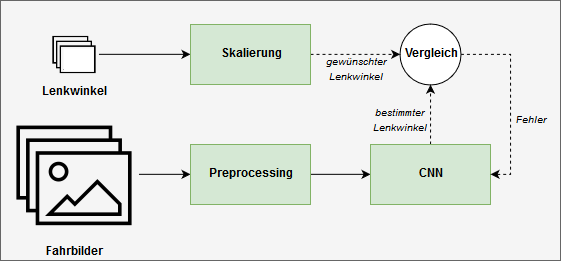
\includegraphics[width=\linewidth]{figures/Lernarchitektur.png}
	\caption{Struktur des Lernprozesses}
	\label{img:lernarchitektur}
\end{figure}

\newpage

\section{Steuerung}

Um aus der Hardware, also der Fahrzeugplattform und der Software, dem neuronalen Netz, eine Steuerungseinheit zu machen, müssen beide Teile verbunden werden. Hierbei ist besonders die Kommunikation wichtig, die Lenkdaten müssen von der erzeugenden Komponente (CNN) zur ausführenden Komponente (Hardwareabstraktion) übertragen werden. Die Steuerungsarchitektur ist in Abbildung~\ref{fig:steuerung} zu sehen.

Über eine Python Schnittstelle zur ueye-Kamera wird die Kamera konfiguriert und Bilddaten ausgelesen. Nach der bereits besprochenen Vorverarbeitung (Preprocessing) werden die Daten an das neuronale Netz weitergereicht.

Der hier bestimmte Lenkwinkel wird nun zur in C/C++ programmierten Steuerung weitergegeben. Dazu werden \gls{ac:uds} verwendet. Die Kommunikation erfolgt statt über eine IP-Adresse über einen File Deskriptor im Unix Betriebssystem. Ein Stream-Protokoll, entspricht dem Internet Protokoll TCP, nutzt den File-Deskriptor als Kommunikationsendpunkt für die Interprozesskommunikation. Der UDS-Client auf der Python-Seite schickt die Lenkdaten direkt an einen UDS-Server auf der C/C++ Seite. Dabei werden die Daten als UTF-8 kodierte Bytestreams verschickt. Die so erhaltenen Daten werden vom UDS-Server entpackt.

Für die direkte Ansteuerung des Lenkungsservos wird der erhaltene Wert auf zwei Nachkommastellen gekürzt und dann direkt an die Hardware weitergegeben. Es erfolgt keine zeitliche Kontrolle auf Zugehörigkeit einzelner Lenkdaten zu Kamerbildern. Die Steuerung soll möglichst hohen Durchsatz haben um möglichst viele Frames in einer Sekunde zur Lenkwinkelermittung nutzen zu können, daher werden immer die aktuellsten erhaltenen Lenkdaten genutzt. Wird ein Datum nicht übertragen, ist es aufgrund der dynamischen Fahrsituation ohnehin schon weniger als eine Sekunde später nicht mehr zur Lenkung zu gebrauchen.

\begin{figure}[h]
	\centering
	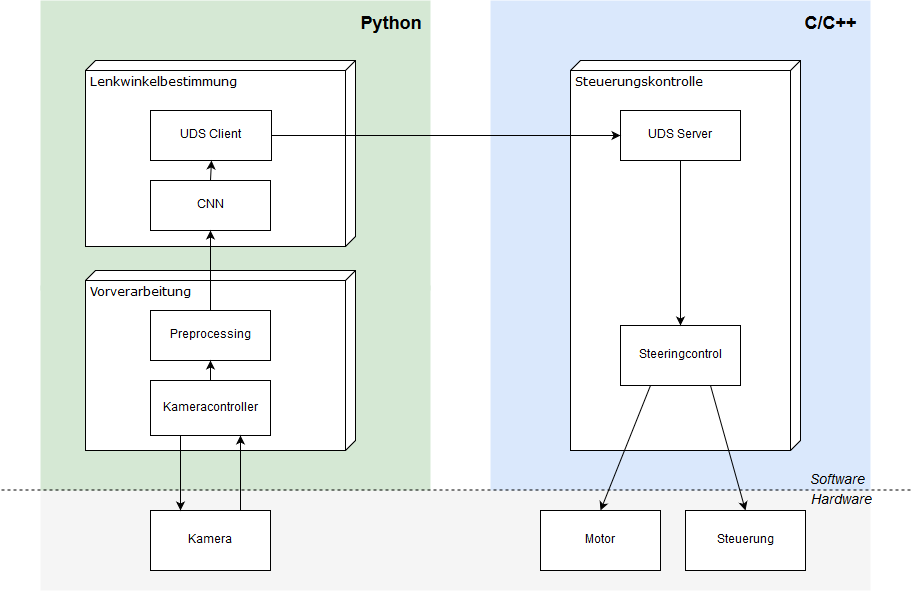
\includegraphics[width=1\linewidth]{figures/Steuerung.png}
	\caption{Komponentenstruktur und Verbindung der Neuronalen Steuerung}
	\label{fig:steuerung}
\end{figure}

Die so gebaute Steuerungskomponente kann zum Fahren des Fahrzeuges verwendet werden. Die Komponenten werden über eine ssh-Verbindung gestartet, die Kontrolle für den autonomen Modus wird dem Fahrzeug über die Funkfernbedienung übergeben. So ist auch ein Eingriff per Hand möglich.

Die Qualität der Steuerung und das Fahrverhalten ist im Weiteren Gegenstand einer Analyse, in der auch aufgezeigt wird, welche Fahrbahn-Eigenschaften das neuronale Netz interpretiert.



